%%%%%%%%%%%%%%%%%%%%%%%%%%%%% Define Article %%%%%%%%%%%%%%%%%%%%%%%%%%%%%%%%%%
\documentclass{article}
%%%%%%%%%%%%%%%%%%%%%%%%%%%%%%%%%%%%%%%%%%%%%%%%%%%%%%%%%%%%%%%%%%%%%%%%%%%%%%%

%%%%%%%%%%%%%%%%%%%%%%%%%%%%% Using Packages %%%%%%%%%%%%%%%%%%%%%%%%%%%%%%%%%%
\usepackage[left=1.5cm,right=1.5cm,top=3cm,bottom=3cm]{geometry} % Adjust specific margins here
\usepackage{graphicx}
\usepackage{amssymb}
\usepackage{amsmath}
\usepackage{amsthm}
\usepackage{empheq}
\usepackage{mdframed}
\usepackage{booktabs}
\usepackage{lipsum}
\usepackage{color}
\usepackage{psfrag}
\usepackage{pgfplots}
\usepackage{bm}
\usepackage[spanish]{babel}
\usepackage[utf8]{inputenc}
\usepackage[T1]{fontenc}
\usepackage{colortbl}
\usepackage[table]{xcolor}
\usepackage{pdflscape} % For landscape page
\usepackage{subcaption}
\usepackage{rotating}

%%%%%%%%%%%%%%%%%%%%%%%%%%%%%%%%%%%%%%%%%%%%%%%%%%%%%%%%%%%%%%%%%%%%%%%%%%%%%%%

% Other Settings

%%%%%%%%%%%%%%%%%%%%%%%%%% Page Setting %%%%%%%%%%%%%%%%%%%%%%%%%%%%%%%%%%%%%%%
\geometry{a4paper}

%%%%%%%%%%%%%%%%%%%%%%%%%% Define some useful colors %%%%%%%%%%%%%%%%%%%%%%%%%%
\definecolor{ocre}{RGB}{243,102,25}
\definecolor{mygray}{RGB}{243,243,244}
\definecolor{deepGreen}{RGB}{26,111,0}
\definecolor{shallowGreen}{RGB}{235,255,255}
\definecolor{deepBlue}{RGB}{61,124,222}
\definecolor{shallowBlue}{RGB}{235,249,255}
%%%%%%%%%%%%%%%%%%%%%%%%%%%%%%%%%%%%%%%%%%%%%%%%%%%%%%%%%%%%%%%%%%%%%%%%%%%%%%%

%%%%%%%%%%%%%%%%%%%%%%%%%% Define an orangebox command %%%%%%%%%%%%%%%%%%%%%%%%
\newcommand\orangebox[1]{\fcolorbox{ocre}{mygray}{\hspace{1em}#1\hspace{1em}}}
%%%%%%%%%%%%%%%%%%%%%%%%%%%%%%%%%%%%%%%%%%%%%%%%%%%%%%%%%%%%%%%%%%%%%%%%%%%%%%%

%%%%%%%%%%%%%%%%%%%%%%%%%%%% English Environments %%%%%%%%%%%%%%%%%%%%%%%%%%%%%
\newtheoremstyle{mytheoremstyle}{3pt}{3pt}{\normalfont}{0cm}{\rmfamily\bfseries}{}{1em}{{\color{black}\thmname{#1}~\thmnumber{#2}}\thmnote{\,--\,#3}}
\newtheoremstyle{myproblemstyle}{3pt}{3pt}{\normalfont}{0cm}{\rmfamily\bfseries}{}{1em}{{\color{black}\thmname{#1}~\thmnumber{#2}}\thmnote{\,--\,#3}}
\theoremstyle{mytheoremstyle}
\newmdtheoremenv[linewidth=1pt,backgroundcolor=shallowGreen,linecolor=deepGreen,leftmargin=0pt,innerleftmargin=20pt,innerrightmargin=20pt,]{theorem}{Theorem}[section]
\theoremstyle{mytheoremstyle}
\newmdtheoremenv[linewidth=1pt,backgroundcolor=shallowBlue,linecolor=deepBlue,leftmargin=0pt,innerleftmargin=20pt,innerrightmargin=20pt,]{definition}{Definition}[section]
\theoremstyle{myproblemstyle}
\newmdtheoremenv[linecolor=black,leftmargin=0pt,innerleftmargin=10pt,innerrightmargin=10pt,]{problem}{Problem}[section]
%%%%%%%%%%%%%%%%%%%%%%%%%%%%%%%%%%%%%%%%%%%%%%%%%%%%%%%%%%%%%%%%%%%%%%%%%%%%%%%

%%%%%%%%%%%%%%%%%%%%%%%%%%%%%%% Plotting Settings %%%%%%%%%%%%%%%%%%%%%%%%%%%%%
\usepgfplotslibrary{colorbrewer}
\pgfplotsset{width=8cm,compat=1.9}
%%%%%%%%%%%%%%%%%%%%%%%%%%%%%%%%%%%%%%%%%%%%%%%%%%%%%%%%%%%%%%%%%%%%%%%%%%%%%%%

%%%%%%%%%%%%%%%%%%%%%%%%%%%%%%% Title & Author %%%%%%%%%%%%%%%%%%%%%%%%%%%%%%%%
\title{Singularidades en las Curvas Poblacionales en el AMBA 1991-2022}
\author{Fernando Meseri}
%%%%%%%%%%%%%%%%%%%%%%%%%%%%%%%%%%%%%%%%%%%%%%%%%%%%%%%%%%%%%%%%%%%%%%%%%%%%%%%

\begin{document}
    \maketitle
    Fernando Meseri
\section{ Introducción}
La información estadística que brindan las proyecciones de población es un insumo principal en la implementación de políticas estatales.  Las proyecciones poblaciones es común encontrarlas a nivel País o Provincia, pero resulta particularmente importante poder contar con dichas proyecciones con un mayor nivel de desagregación, municipio/departamento.
En este caso se analiza en particular los municipios del AMBA, Argentina para el período 1991-2022. Las proyecciones del Instituto Nacional de estadísticas y Censos (INDEC) han estimado la población dichos municipios. El valor arrojado para el CENSO 2022 en el caso de La Matanza presenta una desviación importante respecto al error promedio encontrado entre las proyecciones y el valor relevando en el CENSO 2022. A partir del análisis de datos censales y variables indirectas se analiza las curvas poblacionales, el error en las proyecciones INDEC respecto a lo arrojado en el CENSO 2022 así como el caso puntual de La Matanza.
\section{Revisión bibliográfica}
\subsection{Marco Conceptual}
  La información estadística que brindan las proyecciones de población constituye una herramienta fundamental para la planificación de políticas públicas de corto, mediano y largo plazo. Permite estimar demanda potencial de bienes y servicios en distintas áreas como Salud, Educación, entre otras - Instituto Nacional de Estadísticas y Censos (INDEC,2013) [1]. El estado puede de esta forma determinar los recursos presupuestarios necesarios para satisfacer estas demandas. En la provincia de Buenos Aires ciertos aspectos del presupuesto son asignados en base a la población de cada municipio. Es necesario entonces contar con la información 
  en un alto nivel de desagregación espacial(municipios).
  \subsection{Marco Teórico}
  La elaboración de proyecciones de población es una tarea compleja que debe ser realizada a través de un análisis exhaustivo que permita considerar los censos anteriores como también registros vitales y estimaciones de migración. (INDEC,2013) [1]. En general se ha utilizado en método de las componentes para elaborar dichas proyecciones. Mas esta metodología no ha podido ser replicada al nivel de las jurisdicciones más elementales, departamentos, por cuanto la información no es suficientemente confiable y la inestabilidad de la migración interna no admite formulación de hipótesis a mediano plazo. (Álvarez,2001) [2]. Una forma de realizar estas predicciones ha sido mediante métodos matemáticos de extrapolación en base a la información censal previa. (Álvarez,2001) [2].
  El INDEC provee proyecciones de población por departamento para el período 2010-2025(INDEC, 2015) [3], particularmente para todos los municipios del AMBA. Se destaca que el crecimiento de la población en Argentina observado entre 2001 y 2010 a nivel departamental pone en evidencia las diferencias geográficas que existen en la dinámica poblaciones, con un comportamiento heterogéneo.
  
  \subsection{Estado del arte}
  Históricamente se observa conceso en la utilización del Método de las Componentes para la determinación de proyecciones poblacionales a nivel País o Provincia. El mismo contempla el crecimiento poblacional intercensal y proyecta cada una de las variables determinantes de forma independiente -fecundidad, mortalidad y migración (Álvarez,2001) [2].  Ciertamente la Serie de Análisis Demográfico de INDEC utiliza este método para la proyecciones Nacionales y Provinciales (INDEC, 2015) [3]. 
Asimismo, para población de países desarrollados, también se ha utilizado el modelo de regresión logística en este tipo de predicciones (Gupta, Bhattacharya,Chattyopadhyay ,2012) [4]. Pero este modelo tiene ciertas limitaciones cuando se aplica a data censal dispersa en el tiempo, especialmente para países en desarrollo. Generalmente en estos casos las tasas de crecimiento relativo presentan tendencias inusuales, distintas a la tendencia decreciente de la regresión logística. Gupta et al., (2012) proponen modelos simplificados y variantes de Tsoularis and Wallace Model (TWM) que han proporcionado mejores resultados.
A mayor nivel de desagregación se trabaja con métodos alternativos, como puede ser extrapolación matemática, Ratio- Correlation Method, Housing Unit Method, entre otros (Hoque, 2012)[5]. Por otra parte el centro Latinoamericano y Caribeño de Demografía (CELADE) ha promovido la utilización de otras técnicas para mejorar las estimaciones poblaciones derivadas de la extrapolación matemática. Se utiliza la metodología de variables sintomáticas, que permite establecer correlaciones a las tendencias poblacionales con información de variables indirectamente asociadas al fenómeno de crecimiento poblacional, a saber: nacimientos y defunciones, matrícula escolar, permisos de construcción, otros (Álvarez,2001)[2].  
En lo que respecta a técnicas propias de ciencias de datos para análisis de información censal, se desatacan los siguientes usos: la utilización de data mining para búsqueda de patrones en la información censal, predicciones y forecasting utilizando modelos ARIMA e inducción con árboles de decisión (Chawda, Rane, Giri, 2018) [6]. También se destaca el uso de árboles regresión y clasificación para el agrupamiento o clustering en distintas clases, tomando como input información censal.

\section{Definición del problema }
El municipio de La Matanza una singularidad en su curva de crecimiento poblacional, tanto número de habitantes como tasas intercensales, respecto a los 
municipios aledaños del AMBA para el período 1991-2022.-  
\section{Justificación del estudio}
La información estadística que brindan las proyecciones de población constituye una herramienta fundamental para la planificación de políticas públicas de corto, mediano y largo plazo. Permite estimar demanda potencial de bienes y servicios en distintas áreas como Salud, Educación, entre otras - Instituto Nacional de Estadísticas y Censos (INDEC,2013) [1].
Las proyecciones del INDEC en la serie demográfica N °38(INDEC, 2015) [3] han estimado la población para los municipios del AMBA. El valor arrojado para el censo 2022 en el caso de La Matanza presenta una desviación importante respecto al error promedio encontrado para el resto de los municipios. Es por esto que se pretende analizar la singularidad en la curva poblacional de La Matanza.

\section{ Alcances del trabajo y limitaciones}
El alcance del trabajo es básicamente el análisis y estudio de datos censales. Comprende principalmente la utilización de datos censales del AMBA para el período 1991-2022. Analizar las curvas poblacionales, su comparación y el error en las proyecciones INDEC respecto a lo arrojado en el CENSO 2022 (INDEC ,2022) [7].  El trabajo se limita a demostrar la singularidad o no en el dato poblacional de la Matanza, sin intentar explicar las causas del hecho, particularmente en lo que se refiere al fenómeno 
demográfico que pudiese estar detrás de esta singularidad.
\section{Hipótesis}
Es posible demostrar la curva de crecimiento poblacional de la Matanza presenta una singularidad respecto a los municipios aledaños (AMBA) en situaciones socio-demográficas 
similares para el período 1991-2022. 

\textbf{Preguntas}
\begin{enumerate}
  \item ¿Se puede estimar una tasa de crecimiento promedio de la población urbana/suburbana en base a los 4 Censos anteriores?
  \item ¿Se puede individualizar tasas de crecimiento distintas por municipio??
  \item ¿Considerando las curvas de crecimiento reales de los municipios y las proyecciones realizadas, dado un intervalo de confianza se puede realmente afirmar que la Matanza presenta una singularidad?
  \item ¿Es esperable que municipios aledaños crezcan poblacionalmente en el mismo orden de magnitud?
  \item La apertura de los datos por edad, sexo y nivel de habitantes en el hogar muestra cierto comportamiento esperable, algún patrón. Se asemeja a los valores encontrado para La Matanza para Censo 2022.-
\end{enumerate}

\textbf{Respuestas}
\begin{enumerate}
  \item Sí, es posible determinar la tasa de crecimiento en función a los censos anteriores, utilizando estadística descriptiva.
  \item Sí, es posible, ya que el censo incluye la desagregación por departamento/municipio. Luego estos se pueden agrupar en sectores de interés, ej. AMBA.
  \item	Si, en principio. Las causas de este fenómeno no son de interés del presente trabajo. El fenómeno demográfico es complejo, multicausal. Aun así, se pueden establecer valores de referencia acordes a la región, donde las características socio-demográficas son similar (conurbano).
  \item	Sí, municipios urbanos suburbanos con iguales características socio-demográficas es esperable que tengan tasas de crecimiento similares.
  \item	5.	Es esperable que estos factures socio-demográficos en grandes muestras muestren patronales similares, o valores semejantes.
\end{enumerate}


\section{Objetivos }
El objetivo del presente trabajo consiste en demostrar que la tasa de crecimiento y curva poblacional de la Matanza desde 1991 hasta 2022 presenta una singularidad respecto a aquella desarrollada por los otros municipios de conurbano bonaerense. Tomando como base los datos obtenidos en los 4 últimos censos nacionales 1991-2001-2010 y 2022.  

\textbf{OBJETIVOS ESPECÍFICOS}
\begin{enumerate}
  \item Procesar y unificar la información censal desde 1991 a 2022 para distintos niveles de granularidad, ya que en algunos casos no se presentan todas las variables.  Se requiere un pre procesamiento y limpieza de datos importante.
  \item Exploratory Data Analysis. Construir las curvas poblaciones y comparaciones geográficas de las mismas. Analizar Data mining patterns.
  \item Realizar proyecciones para población censo 2022 con metodologías tradicionales modernas utilizando las variables en forma individual o combinadas, tomando como base los 3 censos anteriores (1991-2001-2010).
  \item Utilizar data mining para rellenar los tiempos intercensales de las variables de interés.
  \item Realizar proyecciones para el censo 2022 mediante data mining (ARIMA, decision tree regression algoritm, others), utilizando los 3 censos anteriores (1991-2001-2010)
  \item Comparar las curvas censales y su ajuste con las proyecciones realizadas para 2022.-
  \item Determinar el error de las distintas proyecciones para 2022 para todos los municipios, comparar con la situación de la Matanza.  
  \item Inferir si existe alguna metodología que ajuste mejor las proyecciones para el caso del AMBA.
\end{enumerate}
\textbf{Variables}
Se trata de una hipótesis multivariable donde las variables podrían tener una relación causa-efecto sobre el fenómeno analizado.
\begin{enumerate}
  \item \textbf{Población Total}. Variable Dependiente. Cuantitativa. Cantidad de personas que habitan un determinado sector del territorio, en distintos niveles de agregación. INDEC
  \item \textbf{Tasa de Natalidad}. Independiente. Cuantitativa. Refiere a la relación que existe entre el número de nacimientos ocurridos en un cierto periodo y la cantidad total de población existente en el área geográfica. 
  \item \textbf{Tasa de mortalidad}. Independiente. Cuantitativa. Es la proporción de personas que fallecen respecto al total de la población en un período de tiempo, usualmente expresada en tanto por mil (‰) por año.
  \item \textbf{Sexo}. Contextual. Categórica. Sexo de las personas, por nivel de desagregación. INDEC
  \item \textbf{Edad}. Contextual. Cuantitativa. Edad de las personas, por nivel de desagregación. INDEC
  \item\textbf{Nivel educativo}.  Contextual. Categórica Ordinal.  Se refiere al nivel de educación máximo alcanzado por un personal hasta el momento. Primario, secundario, terciario, Universitario. INDEC
  \item \textbf{Cantidad de h abitantes en el hogar}. Contextual. Cuantitativa.  Se determina como la cantidad de personas conviviendo de forma permanente bajo el mismo techo. INDEC
  \item \textbf{Asistencia escolar}. Contextual. Categórica Ordinal.  Refiere a la asistencia o no a establecimientos educativos, desagregados por edad. 
  %\%%%%%%%%%%%%%%%%%%%%%%%%%item  INDICE MASCULINIDAD, DENSIDAD DE POBLACION ETC:.
\end{enumerate}

\section{Metodologías}
%Descripción de funcionamiento de cada método a utilizar (Metodología de variables sintomáticas, Data Mining, etc.)
\subsection{Técnicas }
Para dominio del problema, particularmente debido al nivel de desagregación analizado-departamentos-
se utilizarán las siguientes metodologías en el trabajo.\newline
\textbf{Metodologías Tradicionales}\newline
Metodología de variables sintomáticas (distribución por prorrateo; dist. Proporcional; método de tasas variables,
 correlación de razones, correlación de diferencias, correlación de tasas) (Álvarez,2001) [2].
 \newline El método más sencillo es la \textbf{distribución por prorrateo}, que se
basa en el supuesto de que la distribución de la población en un área
mayor se distribuya entre sus áreas menores en forma idéntica a la
distribución de una variable sintomática. La población del área menor
i en el momento t+n está expresada por:
\begin{equation}
  \underset{\textstyle \text{\footnotesize(i,t+n)}}{P}=\frac{\underset{\textstyle \text{\footnotesize(i,t+n)}}{S}}{\underset{\textstyle\text{\footnotesize(t+n)}}{S}} \times \underset{\textstyle \text{\footnotesize(t+n)}}{P}
\end{equation}
Donde:\newline
t+n es el momento n años posteriores al último censo (momento t)\newline
P (i,t+n) población del área menor i en el momento t+n;\newline
P (t+n) estimación disponible de la población del área mayor en el momento t+n;\newline
S (i, t+n) valor de la variable sintomática del área menor i en el momento t+n;\newline
S (t+n) valor de la variable sintomática del área mayor en el momento t+n.\newline
El método de \textbf{distribución proporcional} supone que la población varía durante un período en
 la misma proporción que lo hace la variable sintomática en el mismo período. La población del área
menor i en el momento t+n se deduce de esta relación contemplando un factor de ajuste (Fa) para
que la suma de las áreas menores coincida con el área mayor:

\begin{equation}
  \underset{\textstyle \text{\footnotesize(i,t+n)}}{P}=\frac{\underset{\textstyle \text{\footnotesize(i,t+n)}}{S}}{\underset{\textstyle\text{\footnotesize(i,t)}}{S}}\times \underset{\textstyle \text{\footnotesize(i,t)}}{P}\times \underset{\textstyle \text{\footnotesize(a)}}{F}
\end{equation}

\begin{equation}
  \underset{\textstyle \text{\footnotesize(a)}}{F}=\frac{\underset{\textstyle \text{\footnotesize(i,t+n)}}{P}}
  {\frac{\underset{\textstyle\text{\footnotesize(i,t+n)}}{S}}{\underset{\textstyle\text{\footnotesize(i,t)}}{S}}
  \times
   \underset{\textstyle \text{\footnotesize(i,t)}}{P} }
\end{equation}
\newline
Donde:\newline
t es el momento del último censo;\newline
t+n es el momento n años posterior al último censo;\newline
P (i,t+n) población del área menor i en el momento t+n;\newline
P (i,t) población del área menor i en el momento t ;\newline
S (i,t) valor de la variable sintomática del área menor i en el momento t ;\newline
S (i,t+n) valor de la variable sintomática del área menor i en el momento t+n;\newline
F a factor de ajuste entre suma de áreas menores estimadas y área mayor.\newline
\newline
El método de las \textbf{tasas vitales de Bogue} consiste en estimar la población de áreas menores
utilizando solamente datos de los registros vitales. Bogue (1950) tomó como supuesto la
existencia de una relación inversa entre las variaciones anuales de las tasas de natalidad y de
mortalidad de las áreas menores y que el desvío de las tasas propias en relación a las tasas del área
mayor permanece constante a través del tiempo. La expresión del modelo es:
\newline
\begin{equation}
  \underset{\textstyle \text{\footnotesize(i,t+n)}}{P}=a \times \frac{\underset{\textstyle \text{\footnotesize(i,t+n)}}{B}}
{\underset{\textstyle\text{\footnotesize(i,t+n)}}{b}} + (1-a)\times
\frac{\underset{\textstyle \text{\footnotesize(i,t+n)}}{D}}
{\underset{\textstyle\text{\footnotesize(i,t+n)}}{d}}
\end{equation}
\newline
Donde:\newline
a es el coeficiente de ponderación entre las dos estimaciones;\newline
b (i,t+n) = [ (B (i, t) / P (i, t)) / (B (•, t) / P (•, t)) ] * (B (•, t+n) / P (•, t+n))\newline
d (i,t+n) = [ (D (i, t) / P (i, t)) / (D (•, t) / P (•, t)) ] * (D (•, t+n) / P (•, t+n))\newline
B es la cantidad de nacidos vivos;\newline
b es la tasa bruta de natalidad;\newline
D es la cantidad de defunciones;\newline
d es la tasa bruta de mortalidad.\newline
% El método de correlación de razones se aplica asumiendo que la evolución de la población
% está correlacionada con la variación de una o más variables sintomáticas. La correlación se estima
% por medio de un modelo de regresión, en tanto que la variación se establece por la razón entre los
% valores de una variable correspondientes a dos fechas. El modelo asume la siguiente forma:
% Y (i,t) = a (0)+ a(1) * X1 (i,t) + ... + a(n) * Xn (i,t) + e(i)
% Donde:
% ( ,0) ( ,0)
% ( , ) ( , )
% ( , ) /
% /
% • •
% =
% P P
% P P
% Y
% i
% i t t
% i t
% ( ,0) ( ,0)
% ( , ) ( , )
% ( , ) /
% /
% • •
% =
% Sj Sj
% Sj Sj
% Xj
% i
% i t t
% i t
% 0 es el momento del penúltimo censo;
% t es el momento del último censo;
% Y(i,t) razón entre la proporción del área menor i en los momentos 0 y t;
% Xj(i,t) razón entre la proporción de la variable sintomática j del área menor i en los
% momentos 0 y t;
% e(i) error de la estimación según el modelo.
% Finalmente la población del área menor i puede ser estimada en el momento t+n , a partir de
% la aplicación del modelo de regresión a las razones de variación de las variables sintomáticas entre
% el momento t y t+n, es decir que:
% ( , )
% ( , )
% ( , )
% ( , ) ( , ) t n
% t t
% i
% i t n i t n P
% P P
% P Y
% • +
% •
% + = + × ×
% Donde:
% Y(i, t+n) razón de variación de la población del área menor i estimada para el período t, t+n
% por el modelo de regresión.Estimación de la poblaciones en áreas menores mediante variables sintomáticas
% 16
% El método de correlación de diferencias es semejante al anterior. La diferencia estriba en
% que la variación se establece por la diferencia entre los valores de una variable correspondientes a
% dos fechas. El modelo asume la siguiente forma:
% W (i,t) = a (0)+ a(1) * Z1 (i,t) + ... + a(n) * Zn (i,t) + e(i)
% Donde:
% W(i,t)= [ P(i,t) / P(•,t) ] - [ P(i,0) / P(•,0) ]
% Zj(i,t)= [ Sj(i,t) / Sj(•,t) ] - [ Sj(i,0) / Sj(•,0) ]
% W(i,t) diferencia entre la proporción del área menor i en los momentos 0 y t;
% Zj(i,t) diferencia entre la proporción de la variable sintomática j del área menor i en los
% momentos 0 y t;
% e(i) error de la estimación según el modelo.
% Finalmente la población del área menor i en el momento t+n será:
% P(i,t+n)= [W(i,t+n) + ( P(i,t) / P(•,t) ) ] * P(•,t+n) ]
% Donde:
% W(i, t+n) diferencia de proporciones del área menor i estimada para el período t, t+n por el
% modelo de regresión
% El método de correlación de tasas es otra variante del modelo de correlación de razones.11
% En este caso, se establece una aproximación exponencial del cambio y, en tal sentido, se toma el
% logaritmo natural de cada razón y se lo divide por el tiempo transcurrido entre los censos tomados
% como referencia . En estos casos, el modelo asume la siguiente forma:
% Y* (i,t) = a (0)+ a(1) * X*1 (i,t) + ... + a(n) * X*n (i,t) + e(i)
% Donde:
% k
% nY
% Y ∗(i,t ) = 1 (i,t)
% k
% nXj
% X ∗ j(i,t) = 1 (i,t)
% k es el tiempo transcurrido entre las dos fechas de referencia.
% 11 La descripción del método de correlación de tasas se basa en Chaves Esquivel (s/f).CEPAL - SERIE Población y desarrollo N° 13
% 17
% Finalmente la población del área menor i puede ser estimada en el momento t+n, a partir de
% la aplicación del modelo de regresión a las tasas de variación de las variables sintomáticas entre el
% momento t y t+n, es decir que:
% [ ]
% ( , )
% ( , )
% ( , ) ( , )
% ( , ) t n
% t t
% Y i t n k i
% i t n P
% P P
% P e
% • +
% •
% + ∗
% + = × ×
% ∗
% Donde:
% e
% [Y*(i, t+n) * k] tasa de variación exponencial de la proporción del área menor i estimada para el
% período t, t+n por el modelo de regresión si hubiese transcurrido k años entre t y t+n.
% Finalmente resta comentar que los tres últimos métodos, basados en correlaciones, pueden
% ser refinados en la medida en que se utilicen variables complementarias para distinguir estratos de
% áreas. De esta manera, se mejoran las estimaciones obtenidas por un modelo único para todas las
% divisiones geográficas en cuestión
 
\textbf{Metodologías Data Mining}
CART, ARIMA, decision tree regression and classification algoritms (Chawda, Rane, Giri, 2018) [6]. 
\subsection{Herramientas }
Como herramientas se contemplan los lenguajes Python y SQL. Los datos se trabajarán en base de datos POSTGRES, para visualización geográfica se utilizará QGIS y OpenJump. En cuento al scripting se gestionará mediante Jupyter Notebooks. 

\section{Referencias bibliográficas}

\begin{enumerate}
  \item  Instituto Nacional de Estadística y Censos - INDEC. (2013). Proyecciones provinciales de población por sexo y grupo de edad 2010-2014. - Instituto Nacional de Estadística y Censos - INDEC, 2013. E-Book. (Vol. 1a ed.).
  %\item Alvarez, G., United Nations. Economic Commission for Latin America and the Caribbean., & CELADE (Organization). División de Población. (2001). Estimación de población en áreas menores mediante variables sintomáticas : una aplicación para los departamentos de la República Argentina (1991 y 1996). Naciones Unidas, CEPAL/ECLAC.
  \item  Instituto Nacional de Estadística y Censos - INDEC. (2015). Estimaciones de población por sexo, departamento y año calendario 2010-2025. (1a. ed.).
  \item Gupta, Arindam , Gupta, Arindam , Gupta, Arindam  (2012).Exploring New Models for Population Prediction in Detecting Demographic Phase Change for Sparse Census Data
  \item  Hoque, Nazrul(2012). Evaluation of small area population estimates produced by Housing Unit, Ratio-correlation, and Component Method II compared to 2000 Census counts. Canadian Studies in Population 39, No. 1–2,  pg. 91-108.
  \item Chawda, Manan, Rane, Rutuja, Giri, Skrinanth(2018) 2nd International Conference on Inventive Communication and Computational Technologies (ICICCT) .Demographic Progress Analysis of Census Data Using Data Mining , pg 1894-1897
  % \item \textbackslash{}.h{INDEC CENSO 2022- $[$Archivo de datos$]$ Recuperado de https://www.censo.gob.ar/index.php/datos_provisionales}
  % \item \textbackslash{https://redatam.org/es}
  % \item \textbackslash{https://redatam.indec.gob.ar/argbin/RpWebEngine.exe/PortalAction?BASE=CPV2010A}
  % \item \textbackslash{https://redatam.indec.gob.ar/argbin/RpWebEngine.exe/PortalAction?BASE=CPV2001ARG}
  % \item  \textbackslash{IGM  Capas SIG - Departamento $[Archivo de datos]$ Recuperado de /https://www.ign.gob.ar/NuestrasActividades/InformacionGeoespacial/CapasSIG}
 \end{enumerate}
 \section{DESARROLLO}

 \section{Obtención de datos desde las fuentes. Consolidación Dataset }
 En primera instancia se busca recopilar los datos de los CENSOS poblacionales correspondientes desde 1991. Es decir Censos 1991, 2001, 2010 y 2022.  En general el INDEC dispone la información en formatos CSV o bien archivos Microsoft Excel  de difícil procesado para su ingesta por parte de un  proceso de ETL.  En primera instancia los archivos no cuentan con estructura de encabezados en la primera línea, presentan descripciones y comentarios en las primeras líneas y no respetan formatos uniformes según la dimensión de análisis de los datos dentro del mismo periodo censal. Por otra parte, el formato de presentación y las variables relevadas se han visto modificadas desde el censo 1991 hasta el 2022. Una vez analizada las variables comunes a todos estos censos, fue necesario un pre-proceso manual de los archivos para lograr uniformidad y consistencia de forma de que sean tomados por el proceso de ETL .
 En cuanto a las variables censales comunes al
  período analizado se toman las indicadas en el cuadro  \ref{variables}.
 

 \begin{table}[htbp]
     \centering
     \caption{Descripcion de Variables}
     \begin{tabular}{|l|p{8cm}|}
         \hline
         \textbf{Variable} & \textbf{Description} \\
         \hline
         Censo & Año del censo indicado como entero de 4 dígitos. \\
         CodigoDepto & Código de 4 dígitos con el INDEC indica los municipios / departamentos censales. \\
         Población & Cantidad de personas que habitan un determinado sector del territorio, en distintos niveles de agregación. \\
         Varones & Cantidad de personas de sexo Masculino. \\
         Mujeres & Cantidad de personas de sexo Femenino. \\
         VivPartTot & Cantidad de viviendas particulares totales para ese nivel de agregación. \\
         VivColectTot & Cantidad de viviendas Colectivas totales para ese nivel de agregación. \\
         IndMasc & Índice de masculinidad. \\
         Superficie & Superficie total del partido a la fecha del censo. \\
         \hline
     \end{tabular}
     \label{variables}
 \end{table}

 Es importante aclarar que existe una base consolidada -REDATAM [9]- con toda la información censal para los censos 2001 y 2010, la misma no está disponible para los censos de 1991 y 2022. REDATAM [9] es un software para procesamiento estadístico especializado en microdatos de censos de población y vivienda, encuestas y estadísticas vitales, desarrollado por el CELADE  -  División de Población de la CEPAL, de las Naciones Unidas.  A su vez esta base sólo puede accederse mediante este software específico, no disponiendo de back ups y en general las salidas de las consultas son también archivos CSV no normalizados que requieren post-proceso.
 \subsection{Dimensión Departamento- Slowly Changing Dimension }
 Al analizar los distintos censos desde 1991 hasta 2022 los departamentos del AMBA han modificado su división político – administrativa. Es decir, se han creado varios partidos nuevos, así como fusionado otros. Esto general que la dimensión departamento cambia a través de los distintos censos. Es por esto que se adopta un enfoque tipo Slowly Changing dimensión tipo 3. Donde se impacta el cambio de departamento, conservando en el registro el valor anterior, de que departamento proviene y la superficie correspondiente asociada. Esto es necesario para poder luego procesar información consistente en cuento a la granularidad analizada. 
 Mismo el INDEC consigna :" Nota: con el fin de posibilitar la comparación entre los Censos 1991 y 2001, los datos que 
 corresponden al año 1991 fueron reprocesados según la división político - administrativa
 vigente al año 2001." [8] INDEC, 2001
 
 En el cuadro \ref{tab:DimDepto} puede verse la dimensión departamento con los campos agregados y los comentarios correspondientes en cada caso.
 


\begin{table}[htbp]
    \centering
    \caption{Dimensión Departamento}
    \small
    \begin{tabular}{|c|c|c|c|c|c|p{5cm}|}
        \hline
        Codigo & Departamento & PartidoFrom & Codigo From & Sup1991 & Sup2001 & Comentarios \\
        \hline
        6028 & Almirante Brown & & & 122.0 & 122.0 & \\
        6035 & Avellaneda & & & 55.0 & 55.0 & \\
        6091 & Berazategui & & & 188.0 & 188.0 & \\
        6260 & Esteban Echeverría & & & 377.0 & 120.0 & (1) Superficie modificada, cede tierras a  Cañuelas y San Vicente y para la creación de Ezeiza y Presidente Perón. Leyes provinciales 11.550 del 20/10/1994 y 11.480 del 25/11/1993.\\
        6270 & Ezeiza &	Esteban Echeverría&	6260&0.0&	223.0&	(2) Se crea con tierras del partido de Esteban Echeverría. Ley provincial 11.550 del 20/10/1994.\\
        6274 & Florencio Varela &&& 206.0 & 190.0 & (3) Sup.modificada, cede tierras a Presidente Perón. Ley 11.480 del 25/11/1993.\\
        6371 & General San Martín  &&& 56.0             & 56.0  &    \\
        6408 & Hurlingham & Morón  & 6568  & 0.0   & 36.0 & (4) Se crea con tierras del partido de Morón. Ley provincial 11.610 del 28/12/1994.  \\
        6410 & Ituzaingó  & Morón  & 6568  & 0.0   & 39.0 & (5) Se crea con tierras del partido de Morón. Ley provincial 11.610 del 28/12/1994.   \\
        6412 & José C. Paz  & General Sarmiento & 6005  & 0.0  & 50.0   & (6) Se crea con tierras del partido de General Sarmiento. Ley provincial 11.551 del 20/10/1994. \\
        6427 & La Matanza  &&& 323.0    & 323.0 &  \\
        6434 & Lanús               &&& 45.0              & 45.0  &             \\
        6490 & Lomas de Zamora    &&& 89.0              & 89.0  &     \\
        6515 & Malvinas Argentinas & General Sarmiento & 6005  & 0.0    & 63.0  & (7) Se crea con tierras del partido de General Sarmiento e incorpora un sector del partido de Pilar. Ley provincial 11.551 del 20/10/1994. \\
        6539 & Merlo             && & 170.0             & 170.0 &   \\
        6560 & Moreno              &&& 180.0             & 180.0 & \\
        6568 & Morón                &&& 131.0             & 56.0  & (8) Superficie  modificada, cede tierras para la creación de los partidos de Hurlingham e Ituzaingó. Ley 11.610 del 28/12/1994.\\
        6658 & Quilmes            && & 125.0             & 125.0 &       \\
        6749 & San Fernando       && & 924.0             & 924.0 &    \\
        6756 & San Isidro         && & 48.0              & 48.0  &    \\
        6760 & San Miguel          & General Sarmiento & 6005  & 0.0 & 80.0 & (9) Se crea con tierras del partido de General Sarmiento. Ley provincial 11.551 del 20/10/1994. \\
        6805 & Tigre            &&   & 360.0             & 360.0 &     \\
        6840 & Tres De Febrero   &&  & 46.0              & 46.0  &      \\
        6861 & Vicente López     &&  & 39.0              & 39.0  &  \\
        6005 & General Sarmiento  && & 196.0             & 0.0   & Desaparece para el año 2001   \\        
     \hline
    \end{tabular}
    \label{tab:DimDepto}
\end{table}

\subsection{Diccionario de Departamentos  } 
Debido a las inconsistencias y falta de normalización de los archivos CSV que provee el INDEC, fue necesaria la creación de un diccionario de departamento asociando las distintas acepciones del nombre de departamento con su correspondiente código para que el proceso de ETL pudiese utilizar los códigos de departamento como clave foránea común a todos los Censos Nacionales. Se encontraron casos donde el mismo departamento figura nombrado con tílde ,  
sin tílde , con espacios o abreviaturas en el campo. De esta forma en la ingesta ( ETL) se buscaba el código de departamento correspondiente, que 
funciona como clave única.

\subsection{Proyecciones INDEC 2010-2025  }
Se incorpora también al conjunto de datos que se analizarán proyecciones realizadas por el INDEC [3] que indican la “Población estimada al 1 de julio de
 cada año calendario por sexo, según partido. Provincia de Buenos Aires. Años 2010-2025”.


\subsection{Componente geográfico }
Con el objetivo de enriquecer el dataset se incorpora una tabla con los polígonos geográficos de cada departamento.
 La misma se obtiene del Instituto Geográfico Nacional (IGM) [10], de donde se obtiene la capa SIG para 
 todos los departamentos de la República Argentina. Luego se cruza con el listado de departamentos del AMBA , generando un dataset con las caracteristicas geográficas 
 sumadas a  los datos censales recopilados desde 1991 a 2022.

\begin{table}[htbp]
    \centering
    \caption{Descripción de Variables Geográficas}
    \begin{tabular}{|l|l|p{8cm}|}
        \hline
        \textbf{Variable} & \textbf{Nombre} & \textbf{Descripción} \\
        \hline
        geom & geometry & Polígono WKT con los límites del departamento \\
        fna & Nombre geográfico & Nombre completo que se utiliza para designar un objeto en un mapa o carta. Está formado por el término genérico y el término específico. Ejemplo: río Mendoza. \\
        gna & Término genérico & Parte del nombre geográfico que indica el tipo de objeto que identifica. Ejemplo: río, monte, glaciar, establecimiento. \\
        nam & Término específico & Parte de un nombre geográfico que acompaña al término genérico y que identifica e individualiza un objeto geográfico determinado. Ejemplo: Paraná en río Paraná; Upsala en glaciar Upsala; Las Marías en establecimiento Las Marías; Esperanza en el caso de bahía Esperanza. \\
        in1 & Código INDEC & Código único de vías de circulación asignado por el Instituto Nacional de Estadística y Censos de la República Argentina. \\
        fdc & Fuente de captura & Identificación del nombre y tipo de fuente utilizada para capturar la información. Puede incluir fecha y otros datos adicionales. \\
        sag & Autoridad de fuente & Nombre de la autoridad responsable de la información utilizada. \\
        \hline
    \end{tabular}
    \label{tab:geo.depto}
\end{table}

En base

\subsection{Herramientas }
Para el guardado y manipulación de los datos se va a trabajar con un base de datos POSTGRES (Local). 
Se desarrollo justamente un proceso de ETL en Python y SQL mediante en primera crear todas las tablas necesarias, 
para luego producir la ingesta ,transformar en caso de que sea necesario, de los diferentes inputs que van a componer el modelo de datos.	


\subsection{Diagrama de entidad relación }

\begin{figure}[htbp]
    \centering
    \includegraphics[width=0.8\textwidth]{img/DER.jpg}
    \caption{Diagrama de Entidad Relación}
    \label{fig:DER}
\end{figure}


\section{Metodologías Aplicadas}




%%%%%%%%%%%%%%%%%%%%%%%%%%%%%%%%
\section{ Análisis exploratorio de datos}
\subsection{Población}
Con sustento en la base de datos "AMBA" ( POSTGRES/POSTGIS) se analizarán los distintos datos recopilados según nivel de agregación.
En primera instancia se  generó un dataset con todos los departamentos del AMBA, sus caracteristicas georgráficas así como los valores
de las variables correspondientes a los censos 1991-2001-2010-2022. 
 
En el cuadro \ref{tab:censos_amba} se puede observar el esquema del dataset .
\begin{table}[htb]
  \centering
  \footnotesize
  \begin{tabular}{|c|c|c|c|c|c|c|c|c|c|c|}
  \hline
    \textbf{\cellcolor[rgb]{0,0.231,0.427}\textcolor{white}{nam}} &
   \textbf{\cellcolor[rgb]{0,0.231,0.427}\textcolor{white}{$cod_depto$}} 
   & \textbf{\cellcolor[rgb]{0,0.231,0.427}\textcolor{white}{anio}} &
   \textbf{\cellcolor[rgb]{0,0.231,0.427}\textcolor{white}{pob}} & 
   \textbf{\cellcolor[rgb]{0,0.231,0.427}\textcolor{white}{var}} & 
   \textbf{\cellcolor[rgb]{0,0.231,0.427}\textcolor{white}{muj}} &
    \textbf{\cellcolor[rgb]{0,0.231,0.427}\textcolor{white}{vivpart}} & 
    \textbf{\cellcolor[rgb]{0,0.231,0.427}\textcolor{white}{vivtotal}} &
     \textbf{\cellcolor[rgb]{0,0.231,0.427}\textcolor{white}{sup}} &
      \textbf{\cellcolor[rgb]{0,0.231,0.427}\textcolor{white}{$ind_masc$}} &
       \textbf{\cellcolor[rgb]{0,0.231,0.427}\textcolor{white}{$dens_pob$}} \\
  \hline
  Almirante Brown & 06028 & 1991 & 450698.0 & 222042.0 & 228656.0 & nan & nan & 157.87 & 97.1 & 2854.87 \\
  Almirante Brown & 06028 & 2010 & 552902.0 & 270247.0 & 282655.0 & 156218.0 & 78.0 & 157.87 & 95.6 & 3502.26 \\
  Almirante Brown & 06028 & 2022 & 585852.0 & 281842.0 & 301779.0 & 184403.0 & 60.0 & 157.87 & 93.4 & 3710.98 \\
  Almirante Brown & 06028 & 2001 & 515556.0 & 252454.0 & 263102.0 & 143543.0 & 88.0 & 157.87 & 96.0 & 3265.70 \\
  Avellaneda & 06035 & 2001 & 328980.0 & 155450.0 & 173530.0 & 117200.0 & 59.0 & 68.54 & 89.6 & 4799.82 \\
  Avellaneda & 06035 & 1991 & 344991.0 & 164243.0 & 180748.0 & nan & nan & 68.54 & 90.9 & 5033.43 \\
  Avellaneda & 06035 & 2010 & 342677.0 & 162264.0 & 180413.0 & 121307.0 & 68.0 & 68.54 & 89.9 & 4999.66 \\
  Avellaneda & 06035 & 2022 & 370939.0 & 174572.0 & 194911.0 & 144988.0 & 64.0 & 68.54 & 89.6 & 5412.01 \\
  Berazategui & 06091 & 2010 & 324244.0 & 158608.0 & 165636.0 & 96029.0 & 37.0 & 268.91 & 95.8 & 1205.77 \\
  Berazategui & 06091 & 2022 & 360582.0 & 173892.0 & 186255.0 & 117699.0 & 37.0 & 268.91 & 93.4 & 1340.90 \\
  ...... &  &  &  &  &  & &  &  &  &  \\ \hline
  \end{tabular}
  \caption{Dataset Censos AMBA}
  \label{tab:censos_amba}
  \end{table}
  
  Se observa en el cuadro \ref{tab:summaryCensos} que existen valores nulos para el valor poblaciones, que se corresponden,
   con los casos de municipios de desaparecen en la reorganización administrativa desde 1991 a 2001. Se destaca también que 
   para el censo 1991 no se detalla el total de viviendas particules y colectivas .

  \begin{table}[htbp]
    \centering
    \caption{Summary de columnas de Censos AMBA}
    \label{tab:summaryCensos}
    \begin{tabular}{llll}
        \toprule
        \textbf{Column} & \textbf{Non-Null Count} & \textbf{Dtype} \\
        \midrule
        nam & 96 & object \\
        cod\_depto & 96 & object \\
        anio & 96 & object \\
        pob & 90 & float64 \\
        var & 90 & float64 \\
        muj & 90 & float64 \\
        vivpart & 72 & float64 \\
        vivtotal & 72 & float64 \\
        sup & 96 & object \\
        ind\_masc & 90 & object \\
        dens\_pob & 90 & object \\
        \bottomrule
    \end{tabular}
\end{table}
  


\subsubsection{Población y densidad en vista geográfica}
% \begin{figure}[htbp]
%     \centering
%     \includegraphics[width=0.45\textwidth]{C:/Users/Fer/ITBA_TFI/QGIS/img/AmbaPob1991.jpg}
%     \caption{Diagrama de Entidad Relación}
%     \label{fig:pob1991}
 
% \end{figure}

% \begin{figure}[htbp]
%     \centering
%     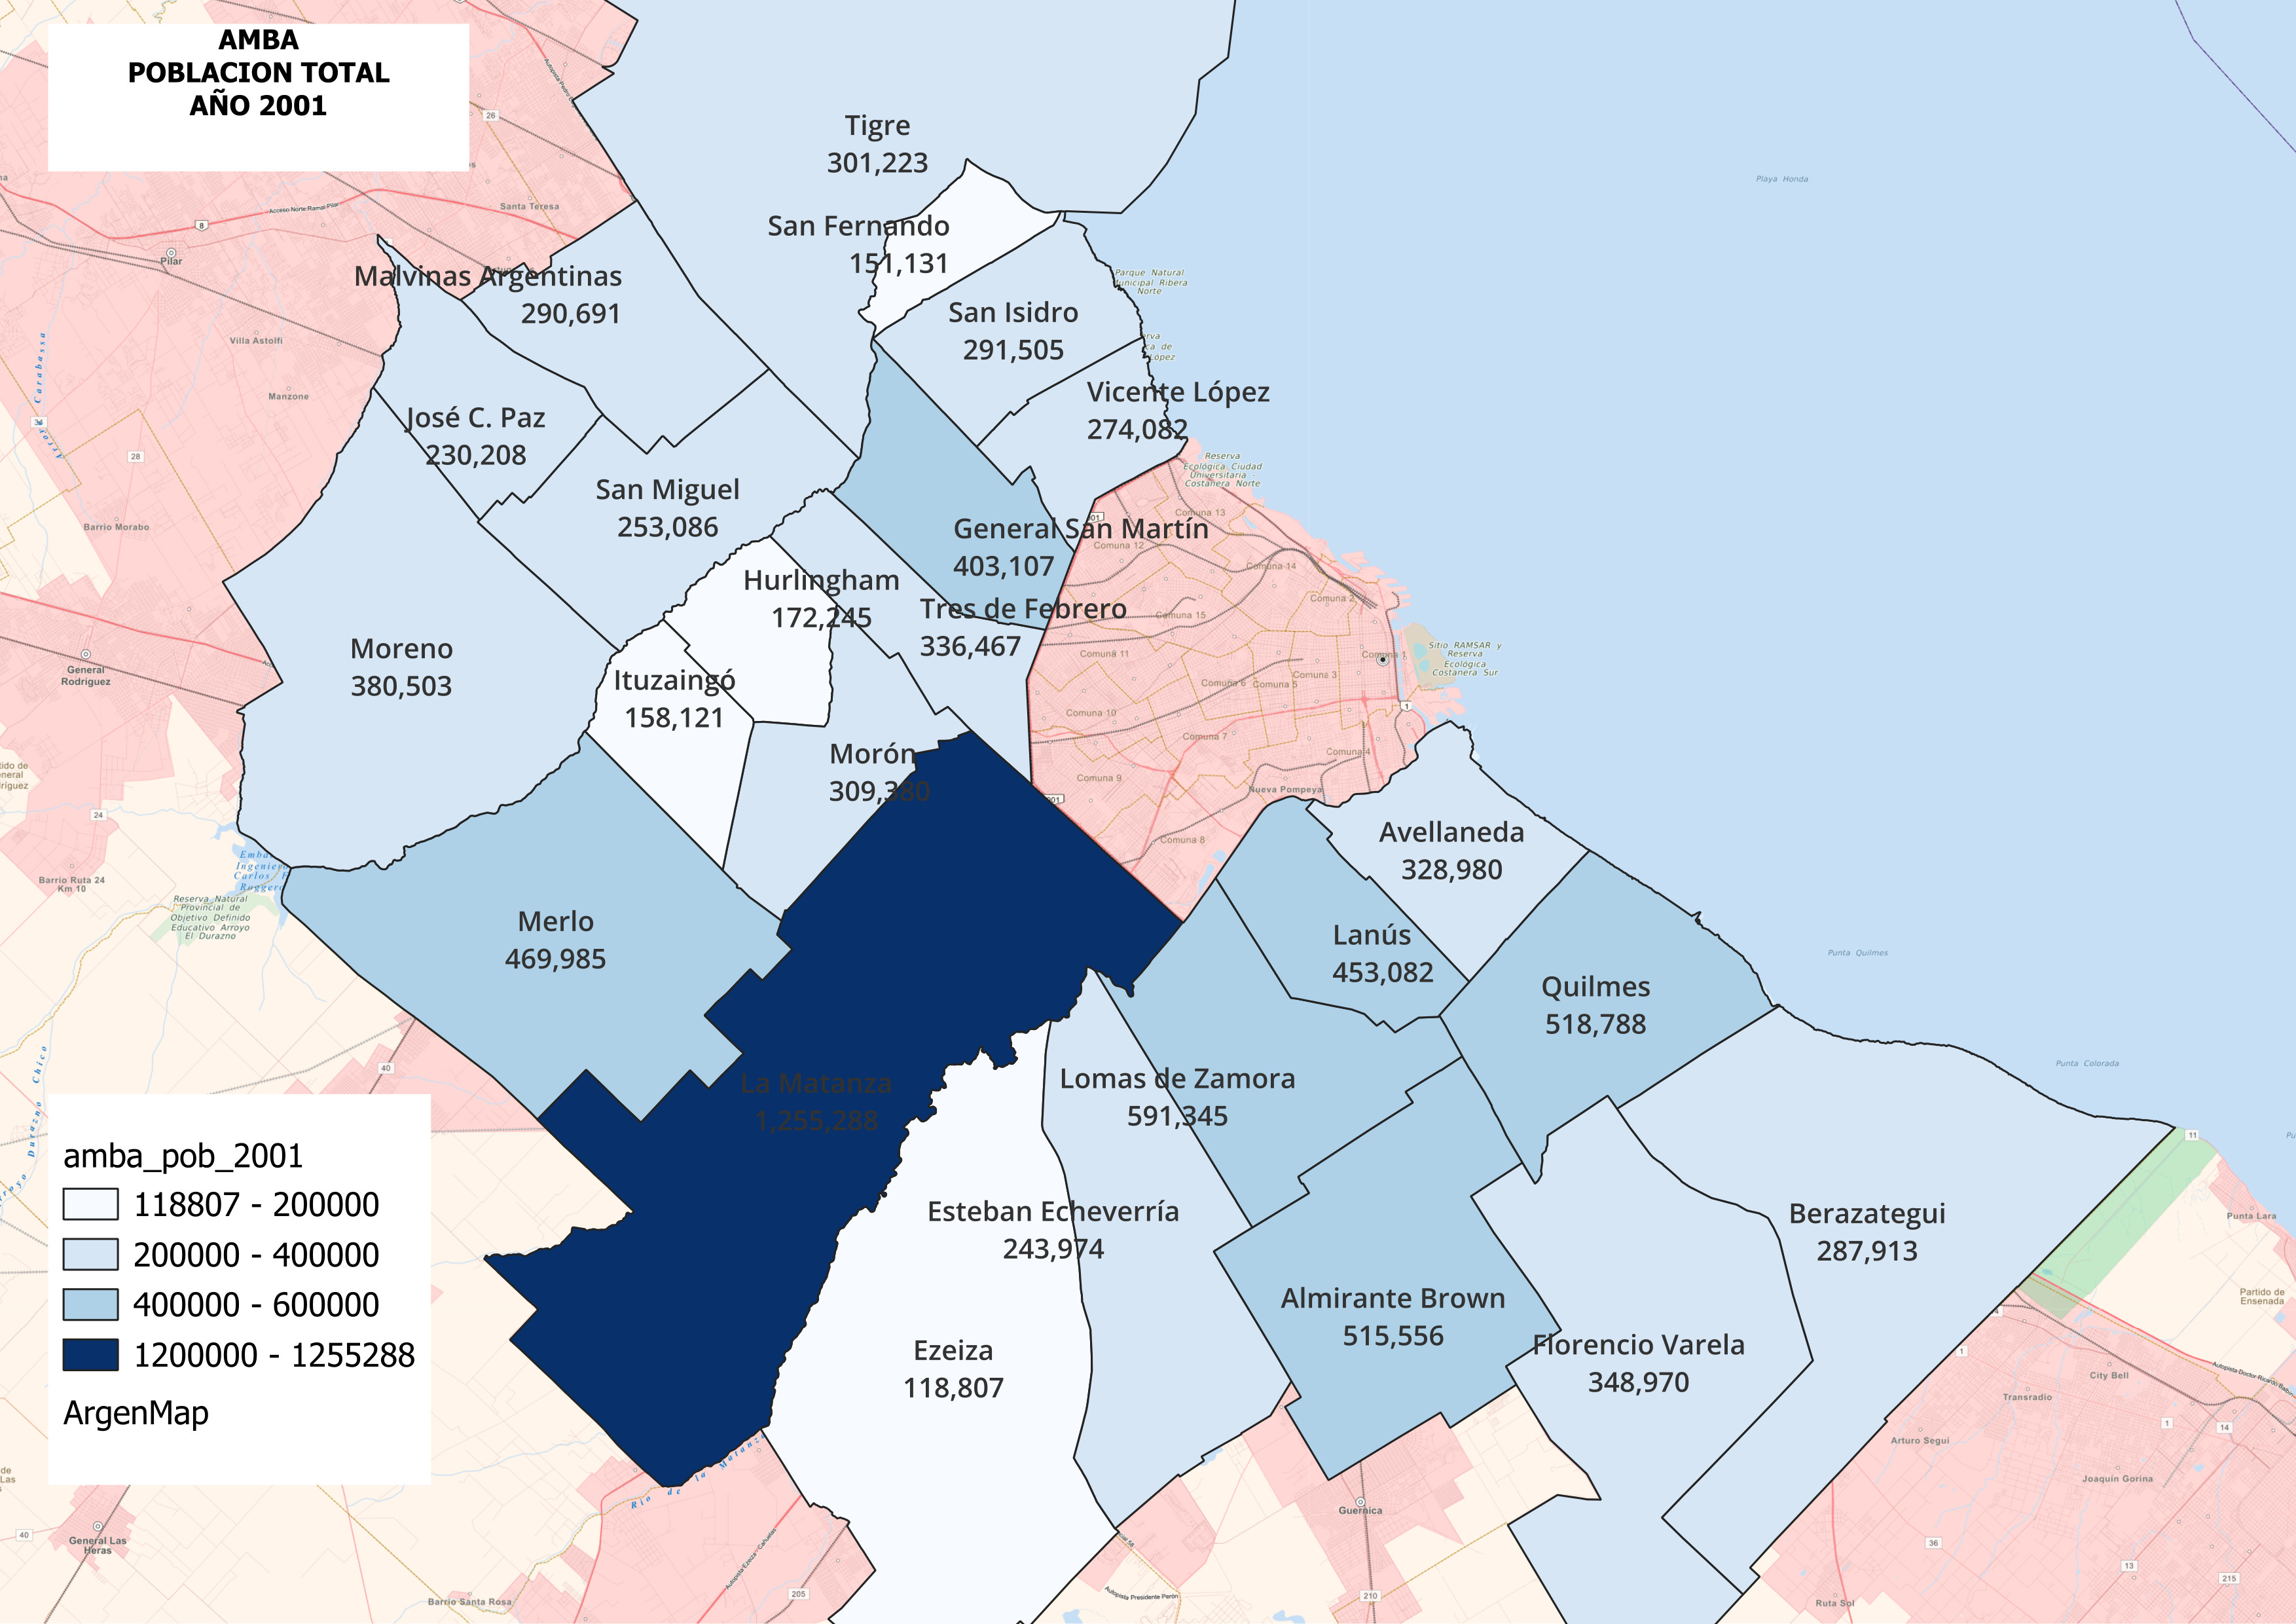
\includegraphics[width=0.45\textwidth]{{C:/Users/Fer/ITBA_TFI/QGIS/img/AmbaPob2001.jpg}}
%     \caption{Diagrama de Entidad Relación}
%     \label{fig:pob2001}
 
% \end{figure}
% \hline
% \begin{figure}[htbp]
%   \centering
%   \includegraphics[width=0.45\textwidth]{C:/Users/Fer/ITBA_TFI/QGIS/img/AmbaPob2010.jpg}
%   \caption{Diagrama de Entidad Relación}
%   \label{fig:pob2010}

% \end{figure}

% \begin{figure}[htbp]
%   \centering
%   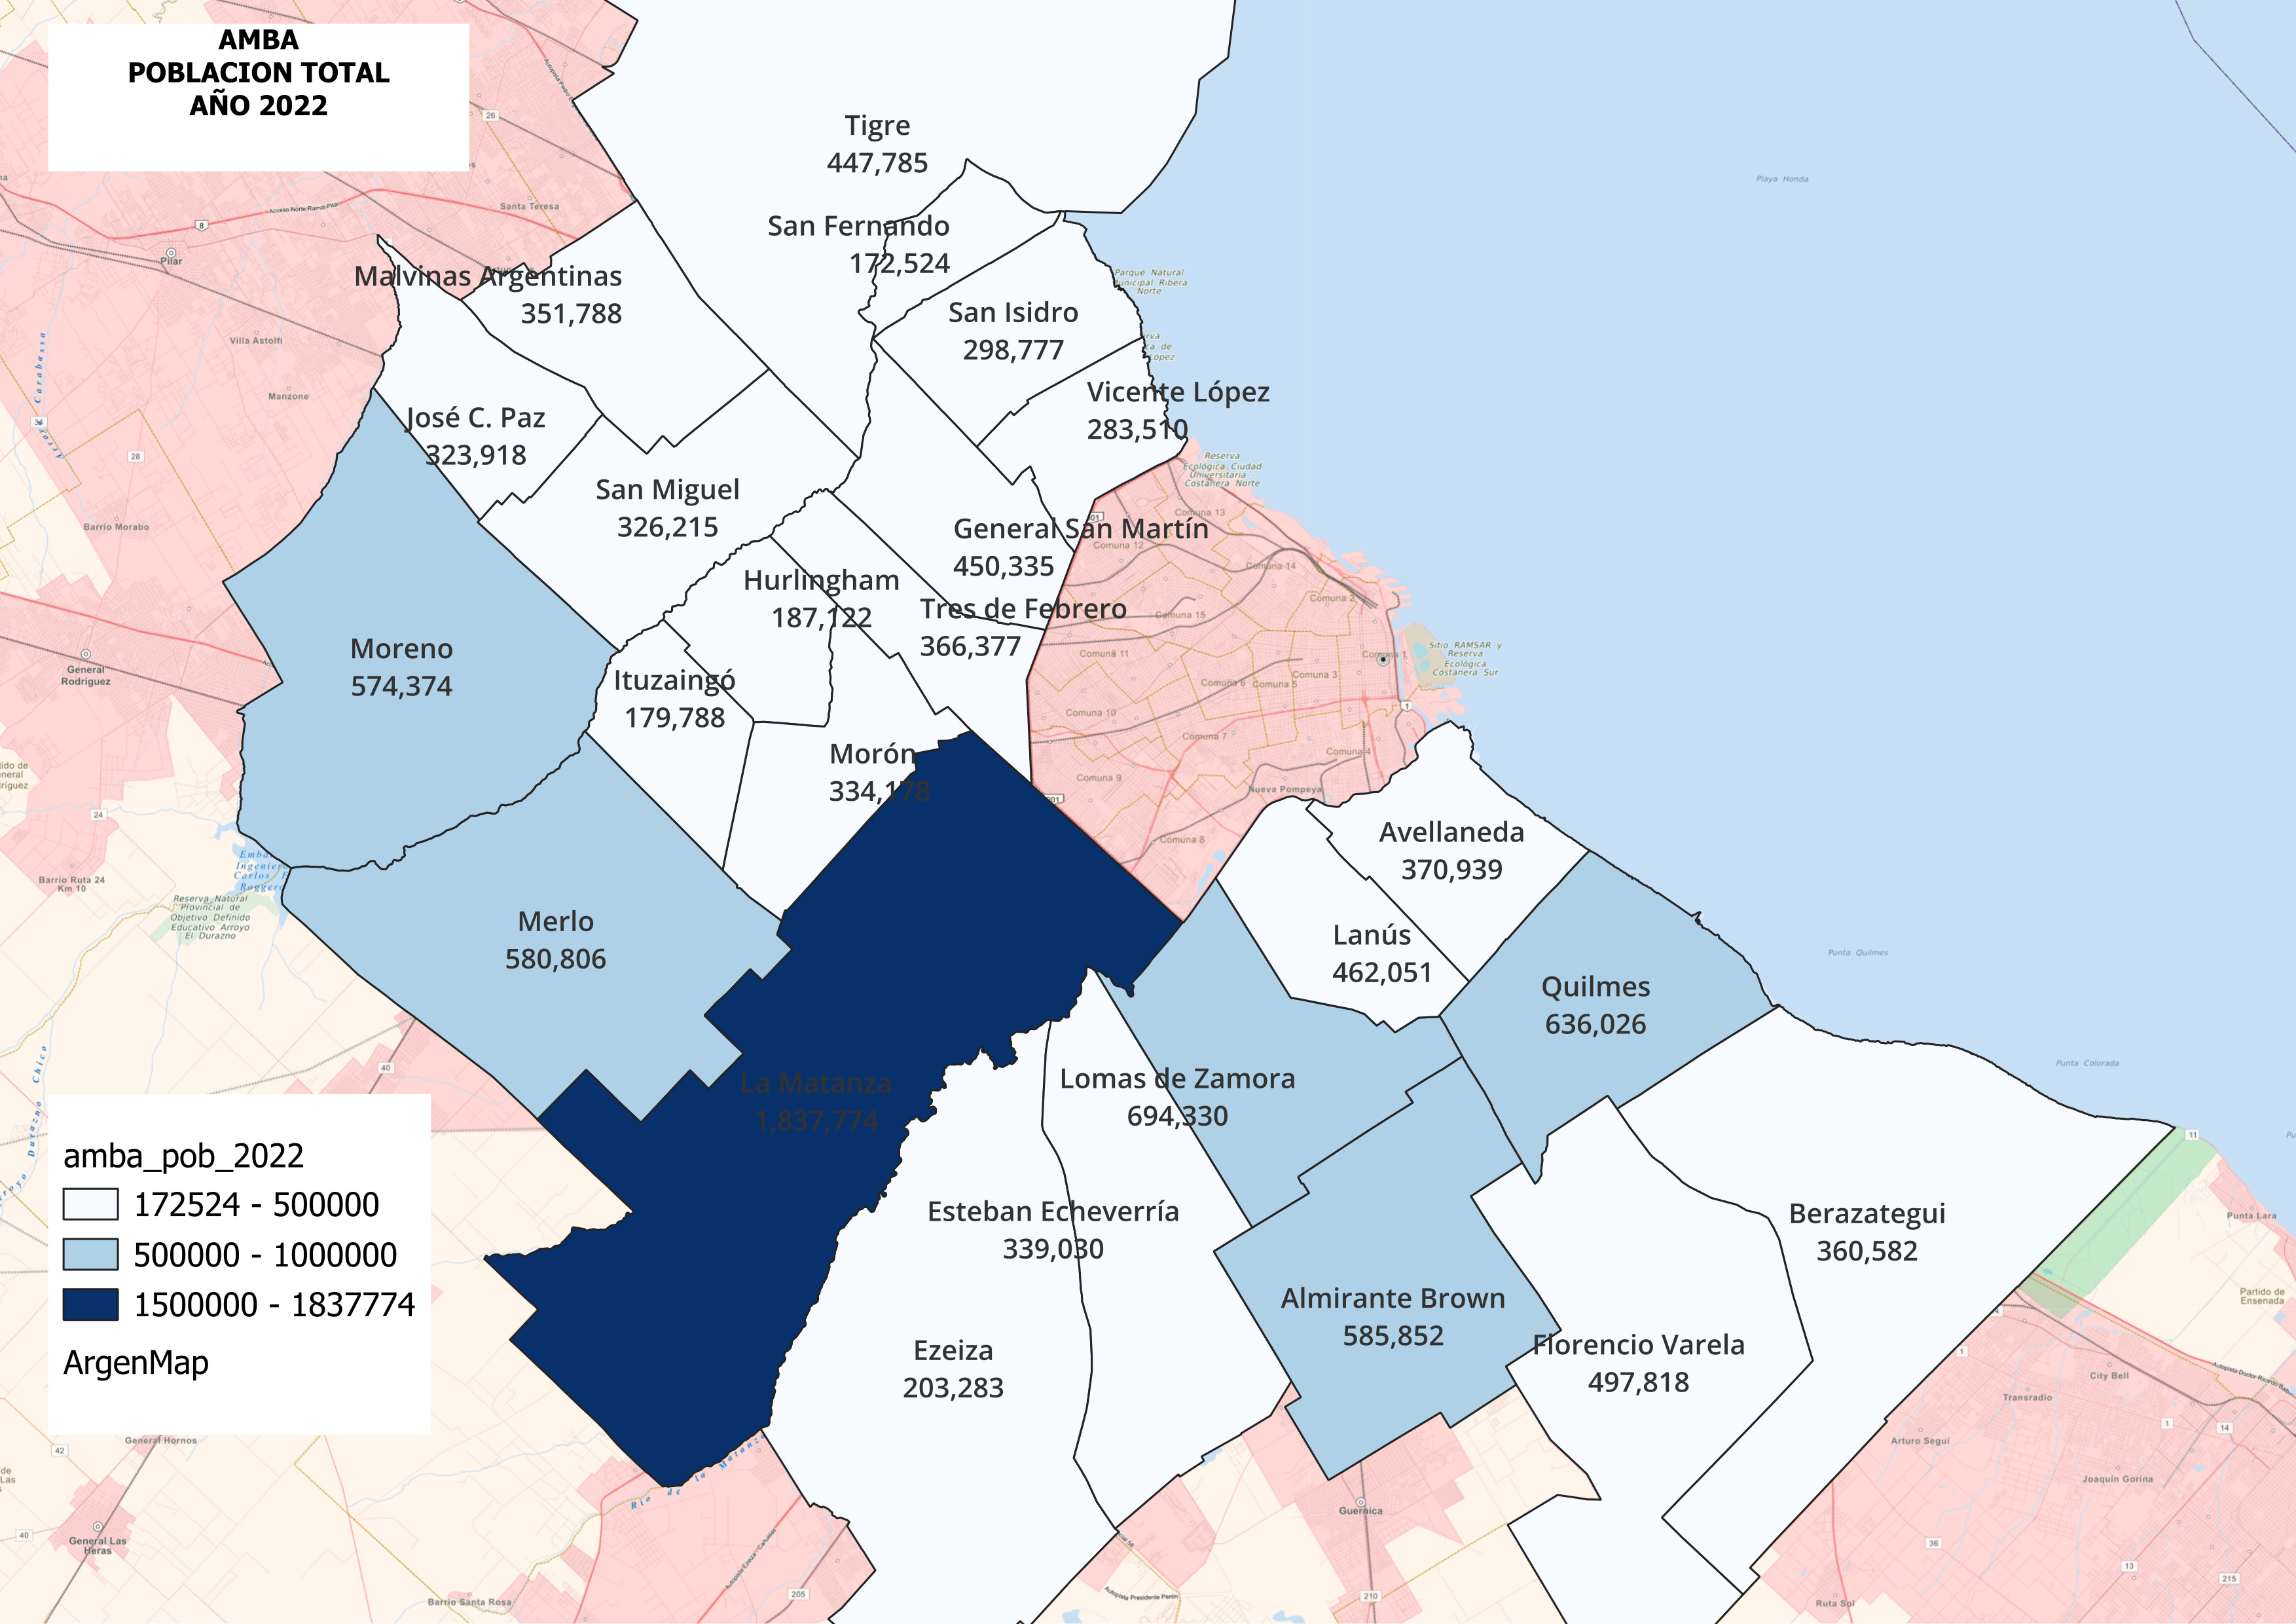
\includegraphics[width=0.45\textwidth]{{C:/Users/Fer/ITBA_TFI/QGIS/img/AmbaPob2022.jpg}}
%   \caption{Diagrama de Entidad Relación}
%   \label{fig:pob2022}

% \end{figure}

\begin{landscape}
\begin{figure}[p] % Use 'p' to force the figures to be placed on a separate page
  \centering
  \begin{subfigure}[b]{0.45\textwidth}
      \centering
      \includegraphics[width=\textwidth]{{C:/Users/Fer/ITBA_TFI/QGIS/img/AmbaPob1991.jpg}}
      \caption{AMBA- Población total Censo 1991}
      \label{fig:pob1991}
  \end{subfigure}
  \quad % Add some horizontal space between subfigures
  \begin{subfigure}[b]{0.45\textwidth}
      \centering
      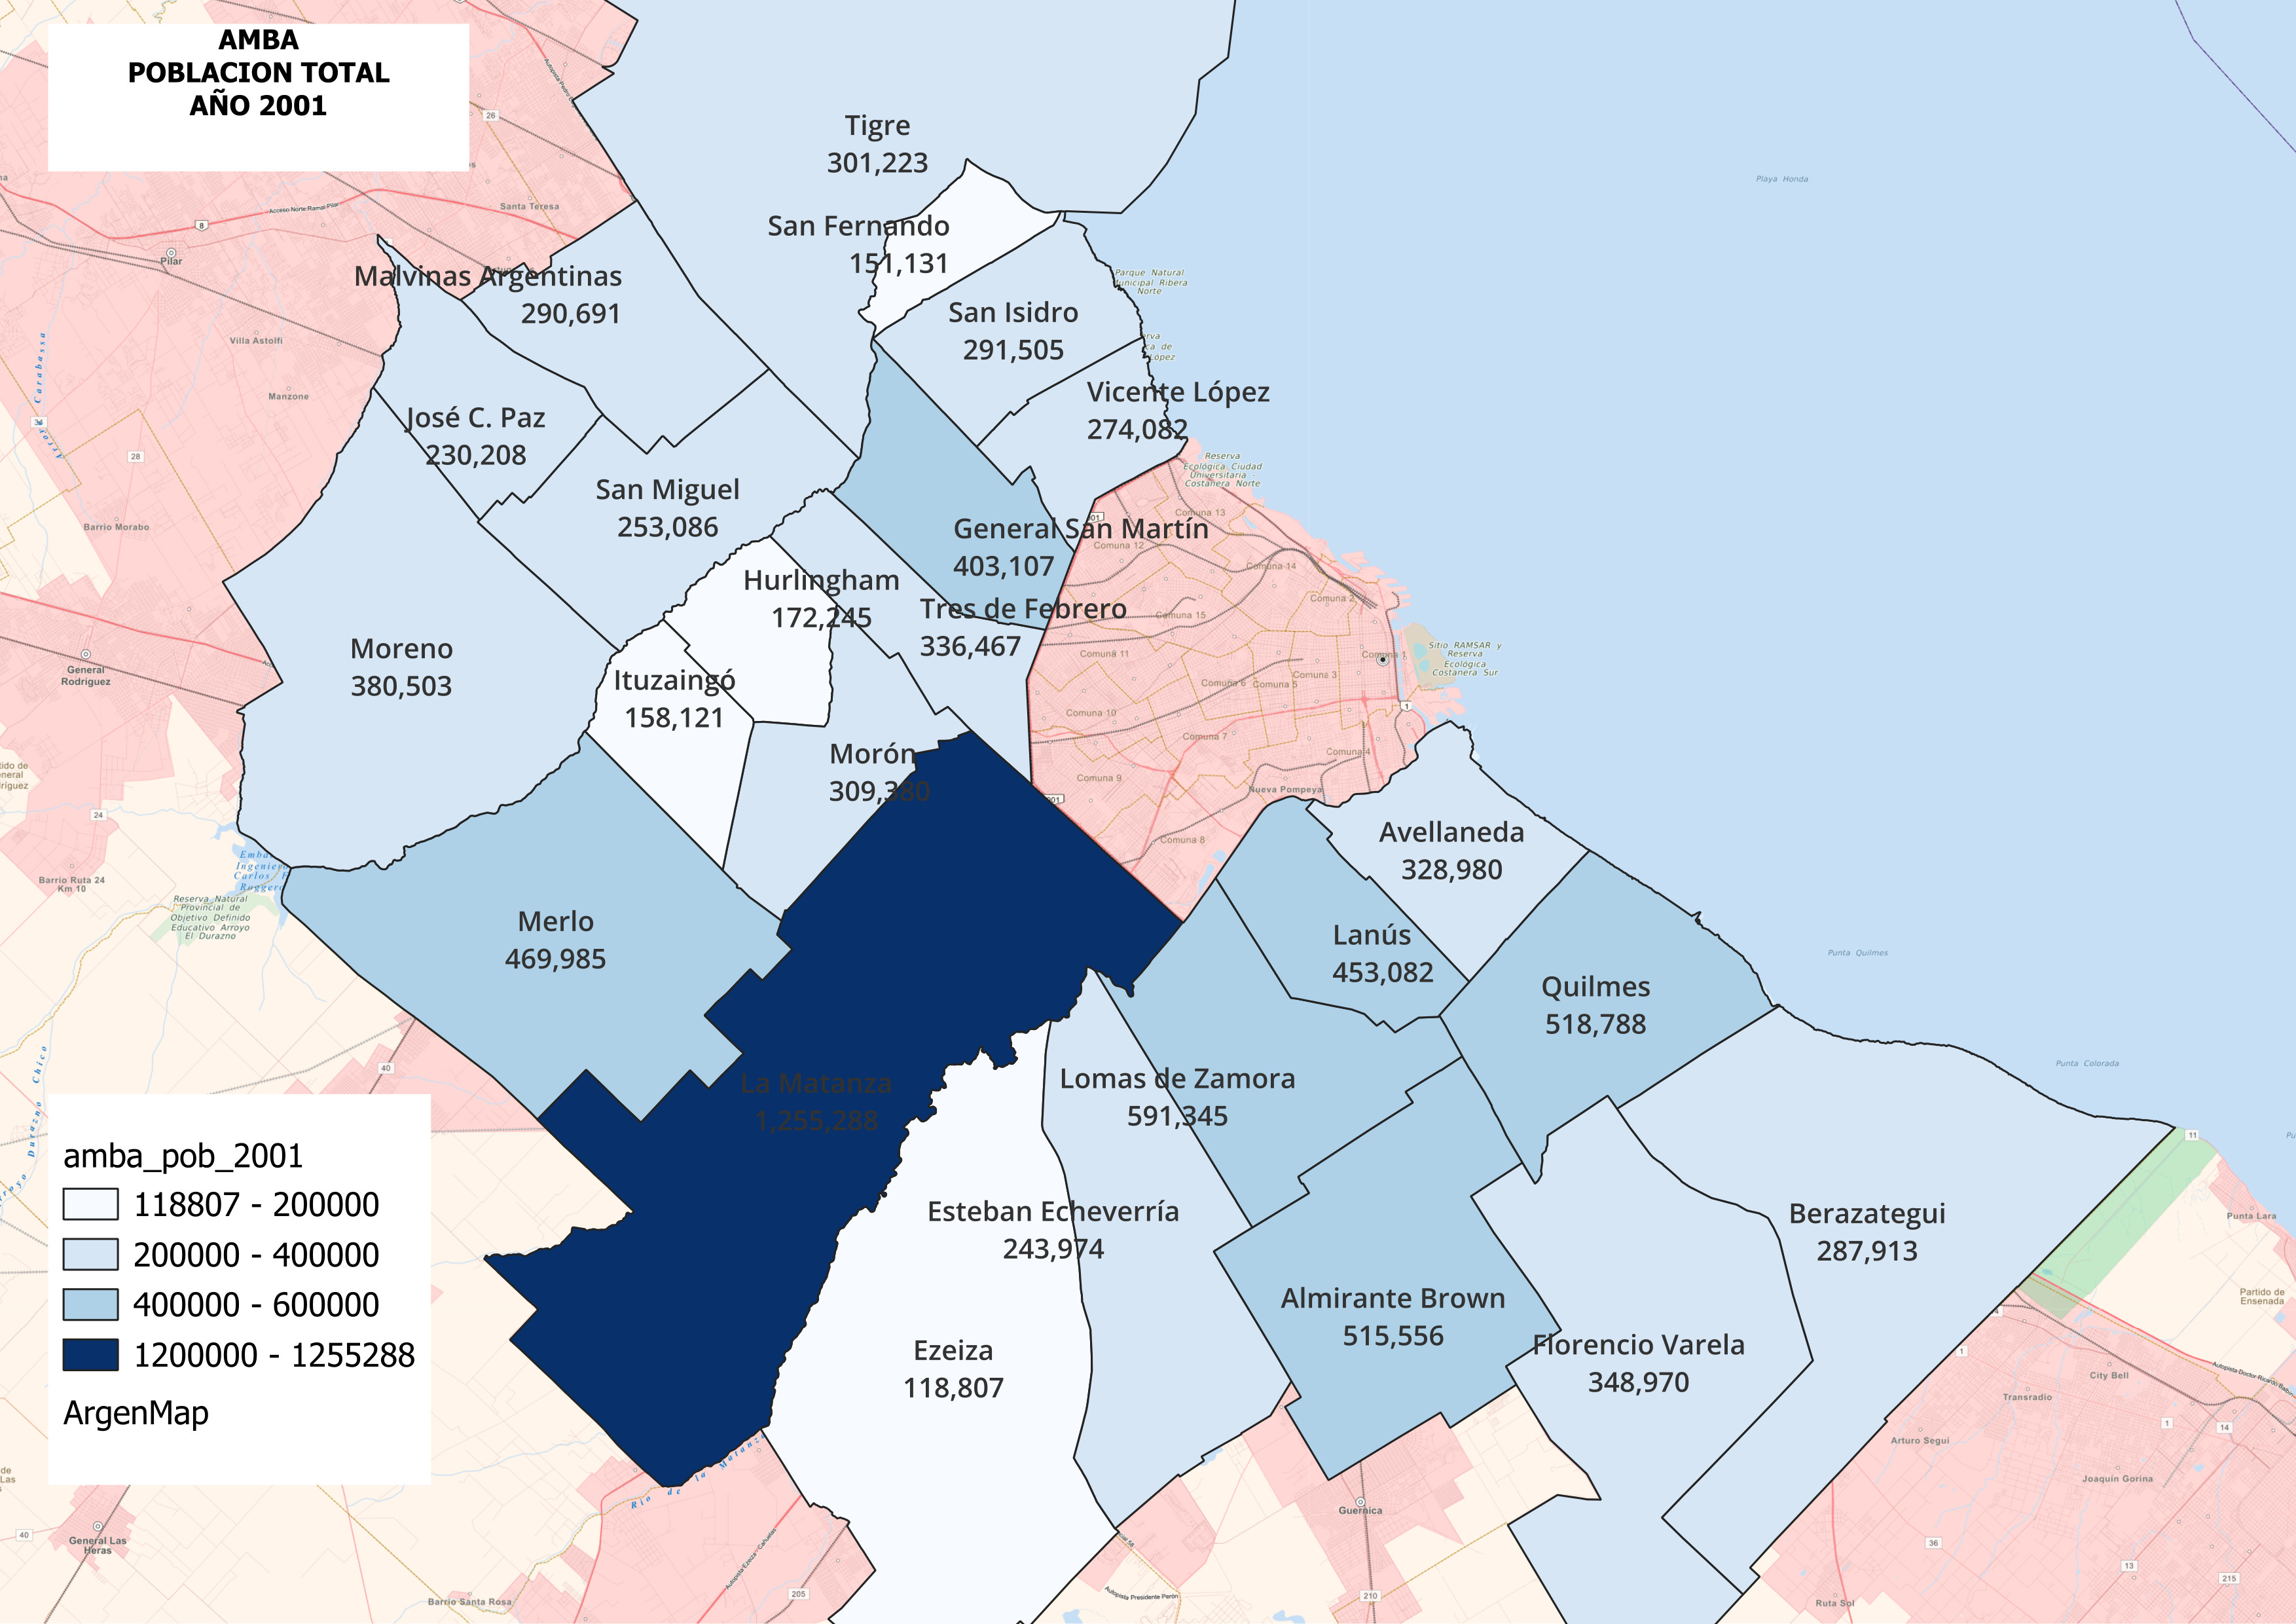
\includegraphics[width=\textwidth]{{C:/Users/Fer/ITBA_TFI/QGIS/img/AmbaPob2001.jpg}}
      \caption{AMBA- Población total Censo  2001}
      \label{fig:pob2001}
  \end{subfigure}
  
  \begin{subfigure}[b]{0.45\textwidth}
      \centering
      \includegraphics[width=\textwidth]{{C:/Users/Fer/ITBA_TFI/QGIS/img/AmbaPob2010.jpg}}
      \caption{AMBA- Población total Censo 2010}
      \label{fig:pob2010}
  \end{subfigure}
  \quad % Add some horizontal space between subfigures
  \begin{subfigure}[b]{0.45\textwidth}
      \centering
      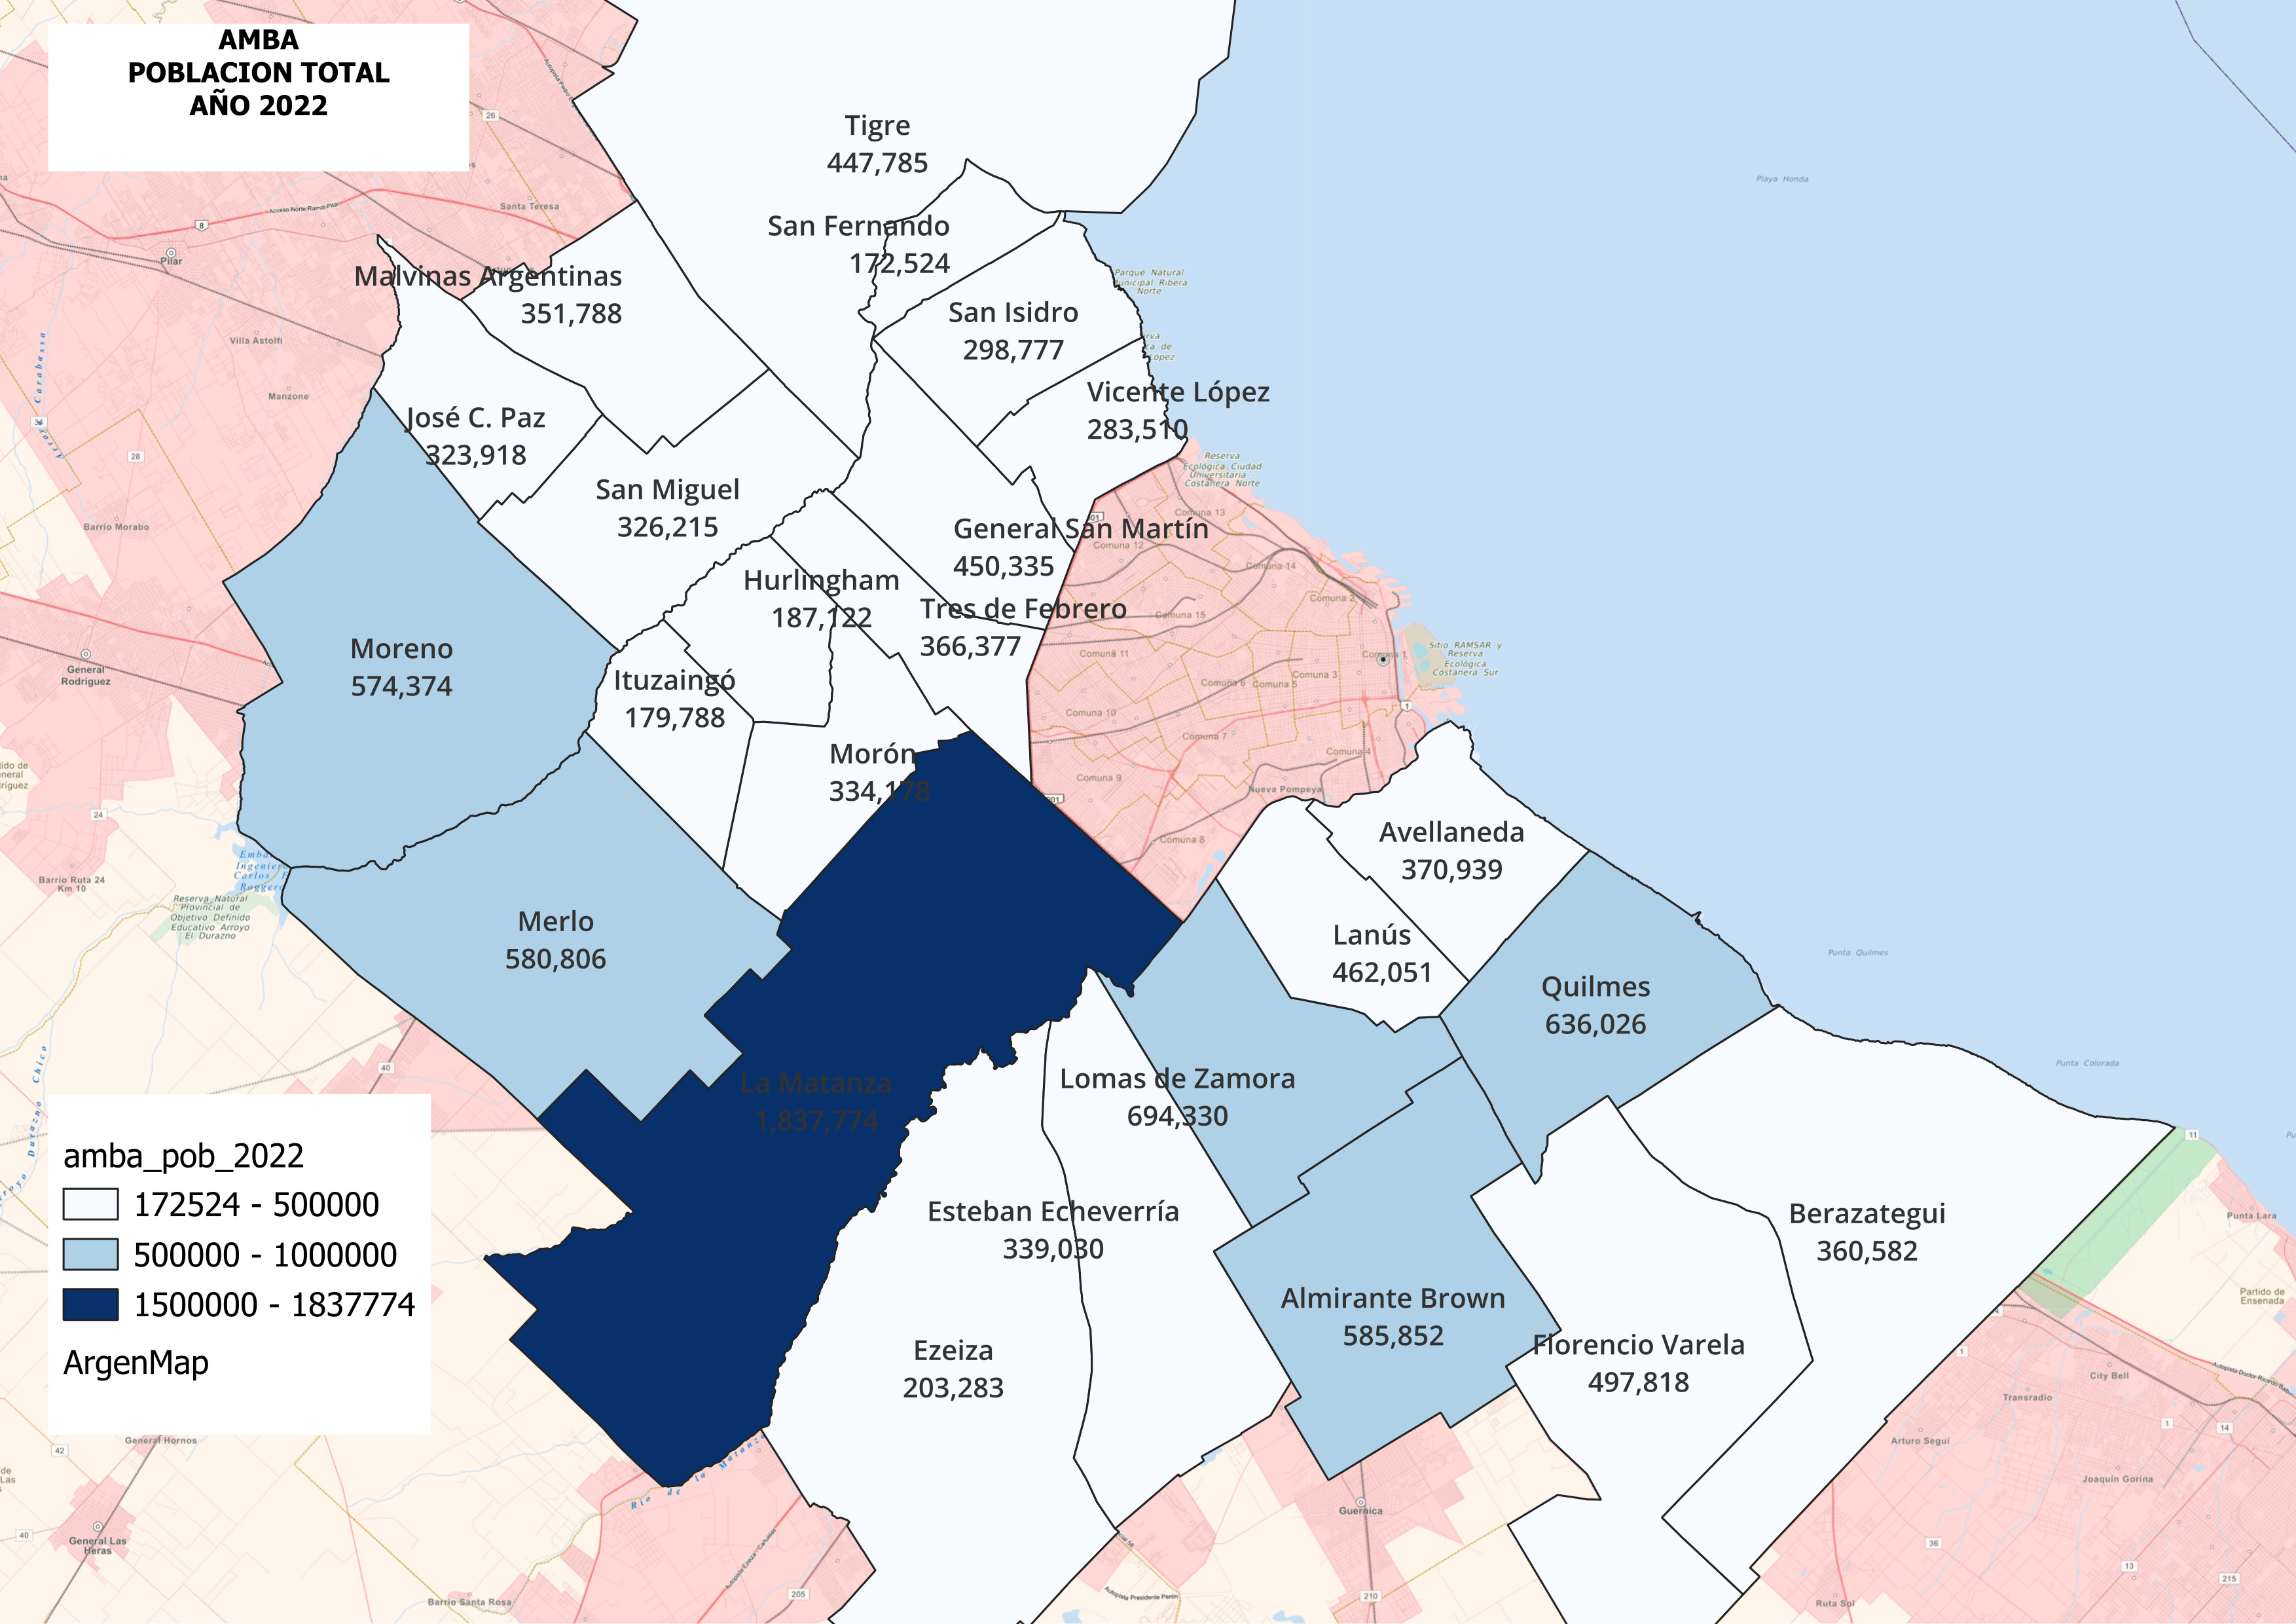
\includegraphics[width=\textwidth]{{C:/Users/Fer/ITBA_TFI/QGIS/img/AmbaPob2022.jpg}}
      \caption{AMBA- Población total Censo 2022}
      \label{fig:pob2022}
  \end{subfigure}
  \caption{Población Total Censos 1991-2022}
  \label{fig:subfigures}
\end{figure}

\end{landscape}

ahora densidad!!!

\begin{landscape}
  \begin{figure}[p] % Use 'p' to force the figures to be placed on a separate page
    \centering
    \begin{subfigure}[b]{0.45\textwidth}
        \centering
        \includegraphics[width=\textwidth]{{C:/Users/Fer/ITBA_TFI/QGIS/img/dens1991.jpg}}
        \caption{AMBA- Población total Censo 1991}
        \label{fig:dens1991}
    \end{subfigure}
    \quad % Add some horizontal space between subfigures
    \begin{subfigure}[b]{0.45\textwidth}
        \centering
        \includegraphics[width=\textwidth]{{C:/Users/Fer/ITBA_TFI/QGIS/img/dens2001.jpg}}
        \caption{AMBA- Densidad [hab/km2] Censo  2001}
        \label{fig:dens2001}
    \end{subfigure}
    
    \begin{subfigure}[b]{0.45\textwidth}
        \centering
        \includegraphics[width=\textwidth]{{C:/Users/Fer/ITBA_TFI/QGIS/img/dens2010.jpg}}
        \caption{AMBA- Población total Censo 2010}
        \label{fig:dens2010}
    \end{subfigure}
    \quad % Add some horizontal space between subfigures
    \begin{subfigure}[b]{0.45\textwidth}
        \centering
        \includegraphics[width=\textwidth]{{C:/Users/Fer/ITBA_TFI/QGIS/img/dens2022.jpg}}
        \caption{AMBA- Población total Censo 2022}
        \label{fig:dens2022}
    \end{subfigure}
    \caption{Población Total Censos 1991-2022}
    \label{fig:subfigures}
  \end{figure}
  
  \end{landscape}

%  %%%%%%%%%%%%%%%%%%%%%%% 
%  MAIN SECTIONS


%  II.	Descripción de funcionamiento de cada método a utilizar (Metodología de variables sintomáticas, Data Mining, etc.)
% III.	Implementación del ETL para extracción y transformación de datos
% IV.	EDA- Análisis exploratorio y descriptivo de las variables

% V.	Comparación entre los modelos 
% VI.	Conclusiones
% %%%%%%%%%%%%%%%%%%%%%%%%55

\end{document}

